\documentclass{article} 
\usepackage[usenames,dvipsnames,svgnames,table]{xcolor}
\usepackage{hyperref}
\usepackage[usenames]{xcolor}
\usepackage{graphicx}
\usepackage{amsmath}
\usepackage{listings}
\usepackage{nameref}
\usepackage{acronym}
\acrodef{AC}[AC]{aggregate computing}
\acrodef{api}[API]{application program interface}
\acrodef{CAS}[CAS]{collective adaptive system}
\acrodef{cps}[CPS]{cyber-physical system}
\acrodef{ci}[CI]{collective intelligence}
\acrodef{cct}[CCT]{concurrent collective task}
\acrodef{dd}[DD]{decentralization domain}
\acrodef{dbms}[DBMS]{database management system}
\acrodef{dcp}[DCP]{distributed computational process}
\acrodefplural{dcp}[DCPes]{distributed computational processes}
\acrodef{dsl}[DSL]{domain-specific language}
\acrodef{RL}[RL]{reinforcement learning}
\acrodef{ict}[ICT]{information and communication technology}
\acrodef{iot}[IoT]{Internet of Things}
%\acrodef{it}[IT]{information technology}
%\acrodef{oca}[OCA]{overlapping collective activity}
\acrodef{mape}[MAPE]{monitor--analyse--plan--execute}
\acrodef{scr}[SCR]{self-organizing coordination regions}
\acrodef{wsn}[WSN]{wireless sensor network}


\newcommand{\revise}[1]{{#1}}


\RequirePackage[sort&compress,sectionbib,numbers]{natbib}


\def\BibTeX{{\rm B\kern-.05em{\sc i\kern-.025em b}\kern-.08em
    T\kern-.1667em\lower.7ex\hbox{E}\kern-.125emX}}

\usepackage{xr}
\externaldocument[main:]{../paper22-ieee-internet-si-decentralised-systems}
\usepackage{xr-hyper}


\newcounter{reviewer}
\newcounter{comment}[reviewer]

\setcounter{reviewer}{-1} % start with zero
\newcommand{\reviewer}{
\subsection*{\refstepcounter{reviewer}Reviewer \arabic{reviewer}}
}
\newcommand{\reviewerl}[1]{
\subsection*{\refstepcounter{reviewer}\label{#1}Reviewer \arabic{reviewer}}
}
\newcommand{\reviewerlt}[2]{
\subsection*{\refstepcounter{reviewer}\label{#1}#2}
}
\newcommand{\comment}[1]{
	\subsubsection*{\refstepcounter{comment}Reviewer Comment \arabic{reviewer}.\arabic{comment}} %\arabic{reviewer}.
	\colorbox{gray!10}{\parbox[t]{\linewidth}{\setlength{\parskip}{0.5\baselineskip}%
 #1 }}
}
\newcommand{\rcref}[2]{\ref{#1}.\ref{#2}}
\newcommand{\commref}[1]{\ref{#1}}
\newcommand{\commentl}[2]{
	\subsubsection*{\refstepcounter{comment}\label{#1}Reviewer Comment \arabic{reviewer}.\arabic{comment}} %\arabic{reviewer}.
	\colorbox{gray!10}{\parbox[t]{\linewidth}{ #2 }}
}
\newcommand{\edcommentl}[2]{
	\subsubsection*{\refstepcounter{comment}\label{#1}Editor Comment \arabic{comment}}\label{name:#1}
	\colorbox{gray!10}{\parbox[t]{\linewidth}{ #2 }}
}
\newcommand{\reply}[1]{	\\[2pt]
	\textbf{Author response:} 	
	#1
}
\newcommand{\related}[1]{	\\[2pt]
	\textbf{Related comments:} 	
	#1
}
\newcommand{\commentAu}[2]{	\\[2pt]
	\meta{\textbf{#1 comment:} 	
	#2}
}
\newcommand{\action}[1]{	\\[2pt]
	\textbf{Action to address the comment:} 
	#1
}
\newcommand{\corrstart}{\color{red}}
\newcommand{\corrend}{\color{black}}
\newcommand{\correction}[1]{\corrstart #1\corrend{}}
\newcommand{\checkstart}{\color{violet}}
\newcommand{\tocheck}[1]{\checkstart{}#1\corrend{}}

\makeatletter
\renewcommand\p@comment{\thereviewer.}
\makeatother

\newcommand{\meta}[1]{{\color{blue}#1}}
\newcommand{\assigned}[1]{{\color{purple}ASSIGNED TO: \textbf{#1}}}

\newcommand{\revq}[1]{{\emph{\textbf{#1}}}}


\newcommand{\say}[3]{
\noindent\fcolorbox{black}{cyan!20!white}{
\begin{minipage}{\textwidth}
\textbf{{#1}} \textbf{({@}#2)}: #3
\end{minipage}
}
}


\usepackage{cleveref}


\begin{document}

\acused{}

\title{{\Large Revision Letter for} ``Dynamic Decentralization
Domains for the Internet of
Things''}
\author{
Gianluca Aguzzi
\and
Roberto Casadei
\and 
Danilo Pianini
\and 
Mirko Viroli
}

\maketitle

Dear Editors, \newline
Thank you very much for allowing us to further improve our article.
%
We have carefully considered the comments of Reviewer 1, accordingly implemented the following minor revisions:
%
\begin{itemize}
\item clarification of the connection between high-level programming model abstractions and the API (see response to Comment~\ref{r1-abstraction-rephrasing});
\item addition of an introductory sentence at the beginning of Section~3, to clarify the evaluation goals, hence setting the expectations of the reader up-front (see response to Comment~\ref{r1-evaluation-intro});
\item fixing of typos and other minor issues (see response to Comment~\ref{r1-minor}).
\end{itemize}
%
%
We think that with these final corrections our work is ready for publication.
\\ ~ \\

\noindent Sincerely yours,

Gianluca Aguzzi, Roberto Casadei, Danilo Pianini, Mirko Viroli


\raggedbottom

%\section*{Comment and replies}

\pagebreak

\reviewerlt{r0}{Editor's Comments}

\edcommentl{ed-code}{
The reviewers recommend acceptance with minor changes; the authors should consider the comments when making their final draft. Reviewer 1 in particular had detailed suggestions for improvement.
}
\reply{
We are glad the reviewers found merits in our manuscript. We also thank them for their additional comments, that we have seriously taken into account for implementing this minor revision.
}


\pagebreak

\reviewerl{r1}

\commentl{r1-overview}{
Recommendation: Accept If Certain Minor Revisions Are Made

Comments:
The authors made a good effort to address all the main points raised by reviewers in the previous round:
\begin{itemize}
	\item the paper now provides a more clear grounding and positioning of the contribution to the state-of-the-art
	\item the authors did a substantial revision of Section 2 to better delimit the conceptual work from the implemented API; this section now includes two subsections: ``Programming Model'' and ``From Requirements to an API''
	\item the authors revised the code listings with a focus on an example for using the API
	\item to improve the evaluation, the authors introduced a new ``risk level'' metric and added an evaluation focused on spatial tracking; the objective is to convey that the system responds as expected to the spatiality and evolution of the tracked phenomenon
\end{itemize}

}
\reply{ 
We thank the Reviewer for the appreciation of our revisions.
%
}

\pagebreak

\commentl{r1-abstraction-rephrasing}{
That said, the presentations of both the programming model and implemented API are still quite high-level. 
This makes it hard to determine what is really the key takeaway from this paper and how it could be reused. 
This should be easily addressed by further improving the presentation. Some concrete suggestions:

- Section 1 currently introduces both the requirements and how the proposed abstractions are meant to address the requirements; 
to better delimit the contribution of the paper, it could help to limit the discussion in Section 1 to requirements and 
move the discussion related to abstractions to Section 2 when discussing the programming model

- what is also missing is a more clear mapping between the proposed abstractions and their reflection in the API as shown in Figure 2a: what is currently shown in Figure 2a and discussed in the figure's caption is too disconnected from the high-level text in Section 2

A more clear delineation between Section 1 and Section 2 and a clearer tack from the proposed abstractions to the programming model to the API should further strengthen Section 2 (the core contribution section).
}
\reply{
The reviewer is right that the presentation of the relationship between requirements and abstractions in Section 1 must be improved. The presentation was not sufficiently clear about the fact that \emph{abstractions} derive from \emph{needs}, and then we formulate \emph{requirements} in terms of what the abstractions should enable. %Namely, requirements discuss what abstractions are needed. 
As such, presentation of requirements and presentation of abstractions cannot be split. We have revised the beginning of subsection ``Requirements and abstractions'' to make this point clear, as follows:
\begin{quote}
\emph{Given the high-level vision and goals discussed in the previous sections, and with the help of FloodWatch,
 we delineate some \emph{needs} together
 with \emph{abstractions} and corresponding \emph{requirements}, for a programming model 
 aimed at decentralized situation recognition and action.
}
\end{quote}

%Since requirements discuss what abstractions are needed, 
% and what these abstractions should enable, we believe that it is better to keep the presentation of requirements and the presentation of abstractions together. This way, the same paragraph introducing an abstraction can also provide some requirements \emph{on} the abstraction just introduced. We clarify at the beginning of subsection ``Requirements and abstractions'' that we also express requirements \emph{on} the abstractions.


Then, the reviewer is also right that the mapping between abstractions and API needs to be correctly draw. Hence, we have clarified and explicitly pointed out with new sentences in Section~2 the relationship between the elements of the API and the DD/CCT abstractions. The new sentence is as follows:
	\begin{quote}
	Specifically, class \texttt{DistributedSensing} denotes \acsp{dd}; types \texttt{Perception}, \texttt{SituatedRecognition}, and \texttt{Action} model sensing, reasoning, and acting operations, respectively; and \texttt{decentralisedRecognitionAndResponse} encapsulates the logic that creates multiple \acsp{cct} and manages their dynamic partitioning into \acsp{dd}.
	\end{quote}
%
%\meta{RC: done -- pls check}
}

%\meta{ON FIRST POINT
%\\
%RC: mmh, I wouldn't like moving those... but we may just follow his suggestion to ``easily'' address this comment. What do you think?}
%
%\meta{GA: I get the point of the reviewer, perhaps in this way we clarify why we chose this programming model. 
%But I also prefer to maintain the discussion about requirements and abstractions in the same section.
%IHMO in this way we clarify the link between those. 
% }
%
%\meta{
%	DP: and yet, we cannot just do nothing. I propose the following:
%	we do not reshape the contents (the discussion flows quite nicely right now),
%	but we promote "Requirements and abstractions" to a full section,
%	and claim that we this is already helping with better identifying the contributions.
%	Also consider that the goal here is to \emph{not} have a third round of review,
%	we want the editor to approve as-is, so the reply to the editor is the real key here.
%}
%
%\meta{
%ON SECOND POINT
%\\
%RC: how may we address this, i.e., make the mapping abstractions--API more visible? may renaming API elements help?}
%
%\meta{GA: We can add more comments in the API, relating each concept/function with the related abstraction/requirements. Probably, we could rename "Data" to DecentralizationDomain? the problem is then the space \dots
%A UML diagram could help? Something like this: 
%
%\centering
%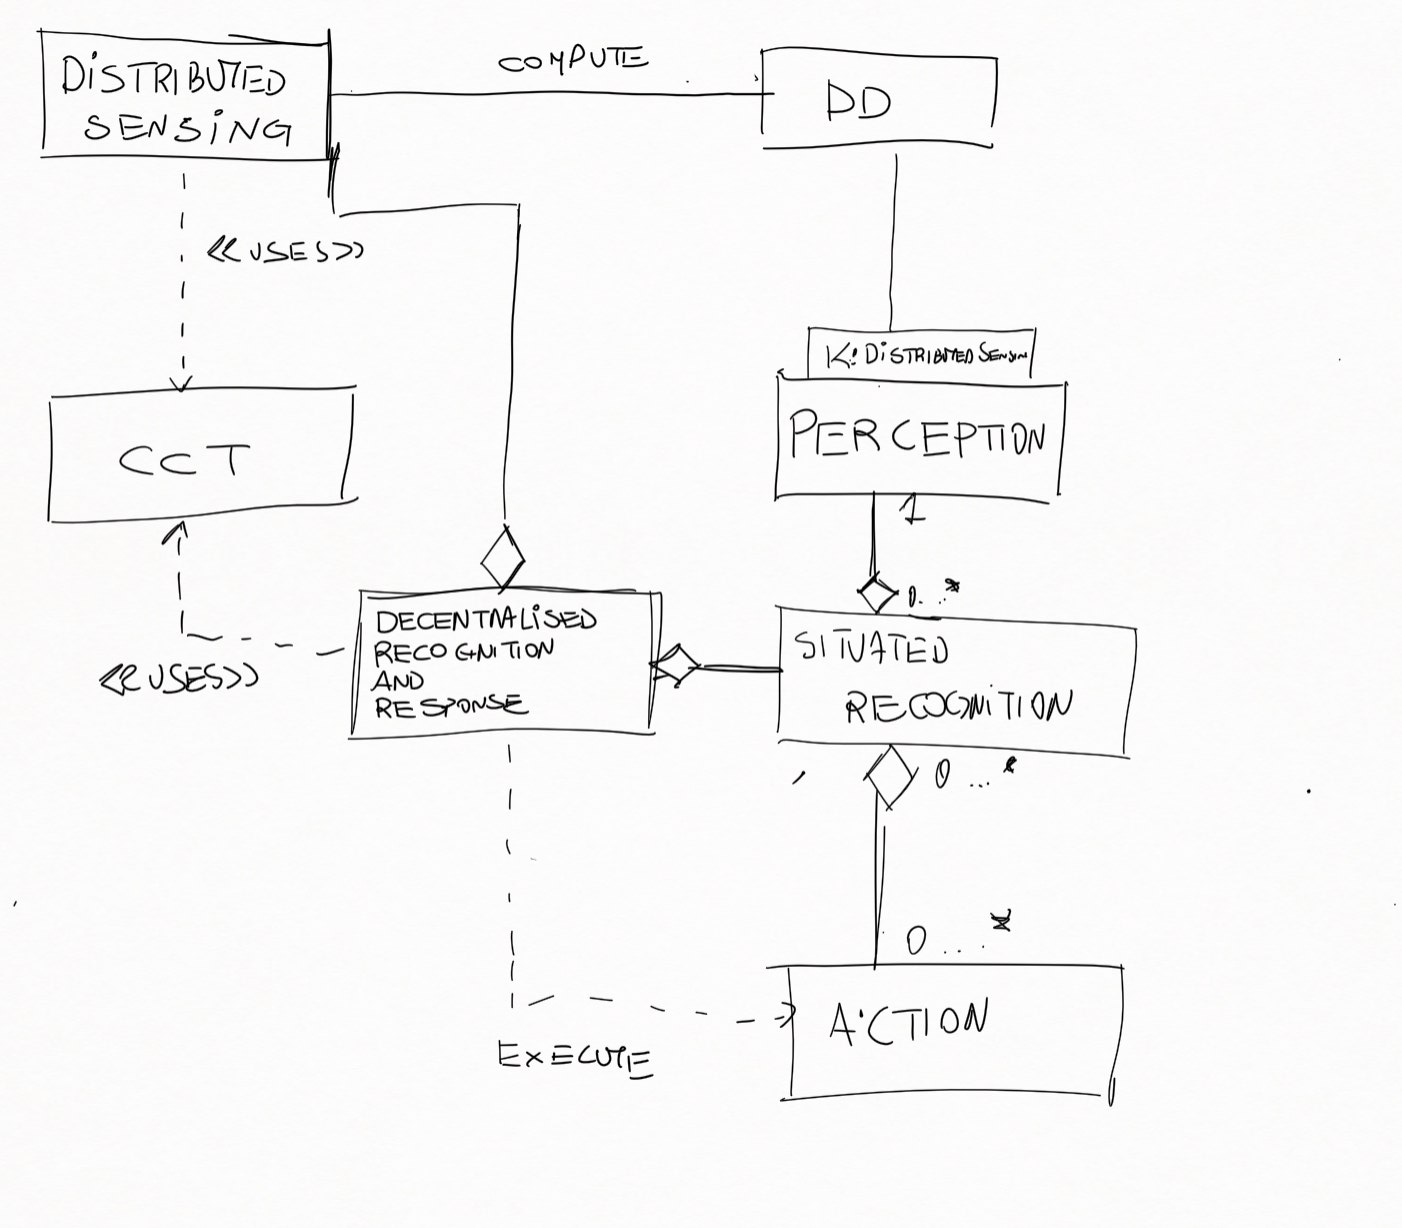
\includegraphics[width=0.99\textwidth]{idea.jpg}
%
%this way, we show the link between the API and the abstractions that we discuss...}
%}

%\commentl{r1-sec1-sec2-delineation}{
%	A more clear delineation between Section 1 and Section 2 and a clearer tack from the proposed abstractions to the programming model to the API should further strengthen Section 2 (the core contribution section).
%}
%\reply{
%We agree that the revisions suggested by Comments~\ref{r1-abstraction-rephrasing} and \ref{r1-figure2-improving} improve Section 2.
%}

\commentl{r1-evaluation-intro}{
	Section 3 (Evaluation) could also benefit from a short introductory paragraph that prepares the reader and sets the right expectations for the evaluation. This section presents a convincing proof-of-concept for a well-developed and realistic scenario. The evaluation is meant to convey to the reader that the abstractions, programming model, and API were successfully used to engineer a system that responds as expected to the underlying phenomenon. This point could be made more explicit to avoid any misunderstanding about performance metrics (because the actual performance of the system is not, in fact, evaluated and it is not the main point of the evaluation)
}
\reply{
An introductory sentence has been added at the beginning of Section~3 as suggested, to clarify the evaluation goals. The new sentence is as follows:
\begin{quote}
\emph{In this section,
 we consider the FloodWatch case study,
 and show that our API
 can successfully be used in a challenging scenario
 to program a system behavior that responds as expected to
 the underlying environmental phenomena.}
\end{quote}
%
%\meta{RC: the reviewer is right: this should be clarified.}
%\meta{RC: done -- pls check}
}

\commentl{r1-minor}{
The above suggestions are only meant to further improve the presentation and should be easily addressed.

Other notes on typos and writing:
\begin{itemize}
	\item page 3, L40-41: ``information from single sensors provides is too fragile''; this phrasing needs to be reviewed

	\item page 4, L52-53: ``CCTs can be thought as a generalisation of''; can be thought of as?

	\item page 6, L39: ``We exercise the examplar in a more challenging''; the example?
\end{itemize}
}
\reply{
Thanks for pointing out these typos: they have been fixed.
}

\commentl{r1-responses}{
	1. How relevant is this manuscript to the readers of this periodical? Please explain your rating in the Detailed Comments section.: Relevant

	2. What is the most appropriate forum for the publication of this manuscript?: IEEE Magazine (general interest explanatory article with technical contributions)
	
	1. Please summarize what you view as the key point(s) of the manuscript and the importance of the content to the readers of this periodical.: The manuscript presents abstractions, a programming model, and API for engineering adaptive decentralized systems that can monitor and react to an underlying phenomenon (e.g., flooding). The contribution was evaluated by implementing a system for a realistic scenario based on open data for rain gauge locations and precipitation in the city of Toronto. The topic is highly relevant for the engineering of IoT systems.
	
	2. Is the manuscript technically sound? Please explain your answer in the Detailed Comments section.: Yes
	
	3. What do you see as this manuscript's contribution to the literature in this field?: - abstractions and a programming model for adaptive decentralized IoT systems; the abstractions build on solid ground and are supported by an API that could potentially be reused
	
	4. What do you see as the strongest aspect of this manuscript?: - the overall narrative is well constructed: it goes from requirements and high-level abstractions to a proof-of-concept based on real data
	
	5. What do you see as the weakest aspect of this manuscript?: - the main contribution section could be further consolidated (see concrete suggestions in my detailed comments)
	
	1. Does the manuscript contain title, abstract, and/or keywords?: Yes
	
	2. Are the title, abstract, and keywords appropriate? Please elaborate in the Detailed Comments section.: Yes
	
	3. Does the manuscript contain sufficient and appropriate references (maximum 15)? Please elaborate in the Detailed Comments section.: References are sufficient and appropriate
	
	4. Does the introduction clearly state a valid thesis? Please explain your answer in the Detailed Comments section.: Yes
	
	5. How would you rate the organization of the manuscript? Please elaborate in the Detailed Comments section.: Satisfactory
	
	6. Is the manuscript focused? Please elaborate in the Detailed Comments section.: Satisfactory
	
	7. Is the length of the manuscript appropriate for the topic? Please elaborate in the Detailed Comments section.: Satisfactory
	
	8. Please rate and comment on the readability of this manuscript in the Detailed Comments section.: Easy to read
	
	9. Please rate and comment on the timeliness and long term interest of this manuscript to IC readers in the Detailed Comments section. Select all that apply.: Topic and content are of immediate and continuing interest to IC readers
	
	Please rate the manuscript. Explain your choice in the Detailed Comments section.: Fair	
}
\reply{
We are glad the Reviewer found merits in our manuscript. The mentioned weakness has been addressed as per the above suggestions.
}

\pagebreak

\reviewerl{r2}

\comment{

Recommendation: Accept If Certain Minor Revisions Are Made

Comments:
Authors have addressed thoroughly the comments raised in the previous round of reviews, and provided an exhaustive response letter.
}
\reply{
	We are glad that the Reviewer appreciated our revisions.
}

\comment{
There are still a few minor issues which should be addressed, such as a typo in line 41 ("provides is"), and a mistake in the caption of Figure 1 (it talks about gray boxes, but there are no gray boxes?). If authors correct these few issues, this reviewer would recommend acceptance.
}
\reply{Thanks for pointing out these typos: they have been fixed.}

\comment{

	Additional Questions:
	1. How relevant is this manuscript to the readers of this periodical? Please explain your rating in the Detailed Comments section.: Very Relevant
	
	2. What is the most appropriate forum for the publication of this manuscript?: IEEE Magazine (general interest explanatory article with technical contributions)
	
	1. Please summarize what you view as the key point(s) of the manuscript and the importance of the content to the readers of this periodical.: The paper proposes two abstractions to model distributed cyber physical systems, namely "concurrent collective tasks" and "decentralization domains". Since the focus is distributed systems that monitor and act on a dynamically changing environment, the content matches the acope of the IEEE Internet Computing Journal.
	
	2. Is the manuscript technically sound? Please explain your answer in the Detailed Comments section.: Appears to be - but didn't check completely
	
	3. What do you see as this manuscript's contribution to the literature in this field?: To this reviewer knowledge, there are no similar abstractions in the literature, so the contribution seems significant and relevant.
	
	4. What do you see as the strongest aspect of this manuscript?: The paper is well written and gives clear examples of applications of the abstractions proposed.
	
	5. What do you see as the weakest aspect of this manuscript?: The paper lacks a more clear formalization of the abstractions. The background on Scala could be expanded.
	
	1. Does the manuscript contain title, abstract, and/or keywords?: Yes
	
	2. Are the title, abstract, and keywords appropriate? Please elaborate in the Detailed Comments section.: Yes
	
	3. Does the manuscript contain sufficient and appropriate references (maximum 15)? Please elaborate in the Detailed Comments section.: References are sufficient and appropriate
	
	4. Does the introduction clearly state a valid thesis? Please explain your answer in the Detailed Comments section.: Yes
	
	5. How would you rate the organization of the manuscript? Please elaborate in the Detailed Comments section.: Satisfactory
	
	6. Is the manuscript focused? Please elaborate in the Detailed Comments section.: Satisfactory
	
	7. Is the length of the manuscript appropriate for the topic? Please elaborate in the Detailed Comments section.: Satisfactory
	
	8. Please rate and comment on the readability of this manuscript in the Detailed Comments section.: Readable - but requires some effort to understand
	
	9. Please rate and comment on the timeliness and long term interest of this manuscript to IC readers in the Detailed Comments section. Select all that apply.: Topic and content are likely to be of growing interest to IC readers over the next 12 months
	
	Please rate the manuscript. Explain your choice in the Detailed Comments section.: Good 
}
\reply{
We are glad the Reviewer found merits in our manuscript.
}

%\bibliographystyle{elsarticle-num}
%\bibliography{../bibliography}

\end{document}
